% Chapter 1
\newpage
\section*{Thesis structure}
\begin{itemize}
    \item Chapter 1: This chapter gives a brief introduction on batteries and the terms associated with understanding a battery technology. Lithium-ion batteries and its shortcomings are discussed, and a comparison between batteries that currently exist in the market is made. Aluminium-ion batteries, both aqueous and non-aqueous, are introduced and ways of finding new cathode materials that can be used in aluminium-ion batteries is explored.
    \item Chapter 2: This chapter explains the experimental methods carried out to assemble a battery on a lab-scale. Procedures for preparing cathode slurries and electrolytes for an aluminum-ion cell have been briefly described.  
    \item Chapter 3: This chapter discusses the characterisation techniques that were implemented post-mortem, to fully analyse how a battery works. Electrochemical processes such as cyclic voltammetry and galvanostatic charge/ discharge curves have been discussed in detail.   
    \item Chapter 4, 5, 6 and 7: These chapters discuss the new materials that were tested as cathodes in aluminium-ion batteries. With a brief review of the literature, new batteries were made using molybdenum dichalcogenides (Chapter 4), carbon-based materials (Chapter 5) and boron nitride/oxide (Chapter 6) as cathodes. Results of several other two-dimensional materials have been reported in Chapter 7. 
    \item Chapter 8: To find cheaper alternatives to the state-of-the-art, new solvents and current collectors were tested while preparing cathodes for aluminium batteries and their performance has been recorded.   
    \item Chapter 9: This chapter summarises the research findings of chapters 4-8 and provides an outlook for future researches. Many new scientific findings have been made, which need to be studied and analysed in greater detail, so that aluminium-ion batteries can find commercial use.
    \end{itemize}
\newpage
\section*{Preface}
This chapter gives a brief introduction on batteries and the terms associated with understanding a battery technology. Lithium-ion batteries and its shortcomings are discussed, and a comparison between batteries that currently exist in the market is made. Aluminium-ion batteries, both aqueous and non-aqueous, are introduced and ways of finding new cathode materials that can be used in aluminium-ion batteries is explored.
\newpage
\chapter{Batteries --- an introduction} % Main chapter title
 \label{chap1} % For referencing the chapter elsewhere, use \ref{Chapter1} 
%----------------------------------------------------------------------------------------
% Define some commands to keep the formatting separated from the content 
\newcommand{\keyword}[1]{\textbf{#1}}
\newcommand{\tabhead}[1]{\textbf{#1}}
\newcommand{\code}[1]{\texttt{#1}}
\newcommand{\file}[1]{\texttt{\bfseries#1}}
\newcommand{\option}[1]{\texttt{\itshape#1}}

%----------------------------------------------------------------------------------------
A lot is being done to switch over to renewable sources of energy from non-renewables to combat climate change. By installing solar panels on their rooftops, consumers are now powering their houses by tapping solar energy. However, solar and wind energies have variable output. The sun doesn't always shine and the wind doesn't always blow. Energy storage is necessary for a continuous power supply. Batteries maximize our ability to use the electricity generated by renewable sources of energy, on a day-to-day basis. Figure \ref{Figures/chap1fig:IEC2} diaplys the data from 2018 generated by International Energy Association (IEA). They store energy in a chemical form, which can be used at a later time. If used in houses, a battery can store the power generated by the sun for several hours. In a grid system, when supply is higher than demand, electricity can be used to power batteries. When demand is higher than supply, stored energy can be used by the grid. To understand how a battery works, it is important that we understand a few terms that are helpful in evaluating its performance. 

\begin{figure}[tbh!]
\centering
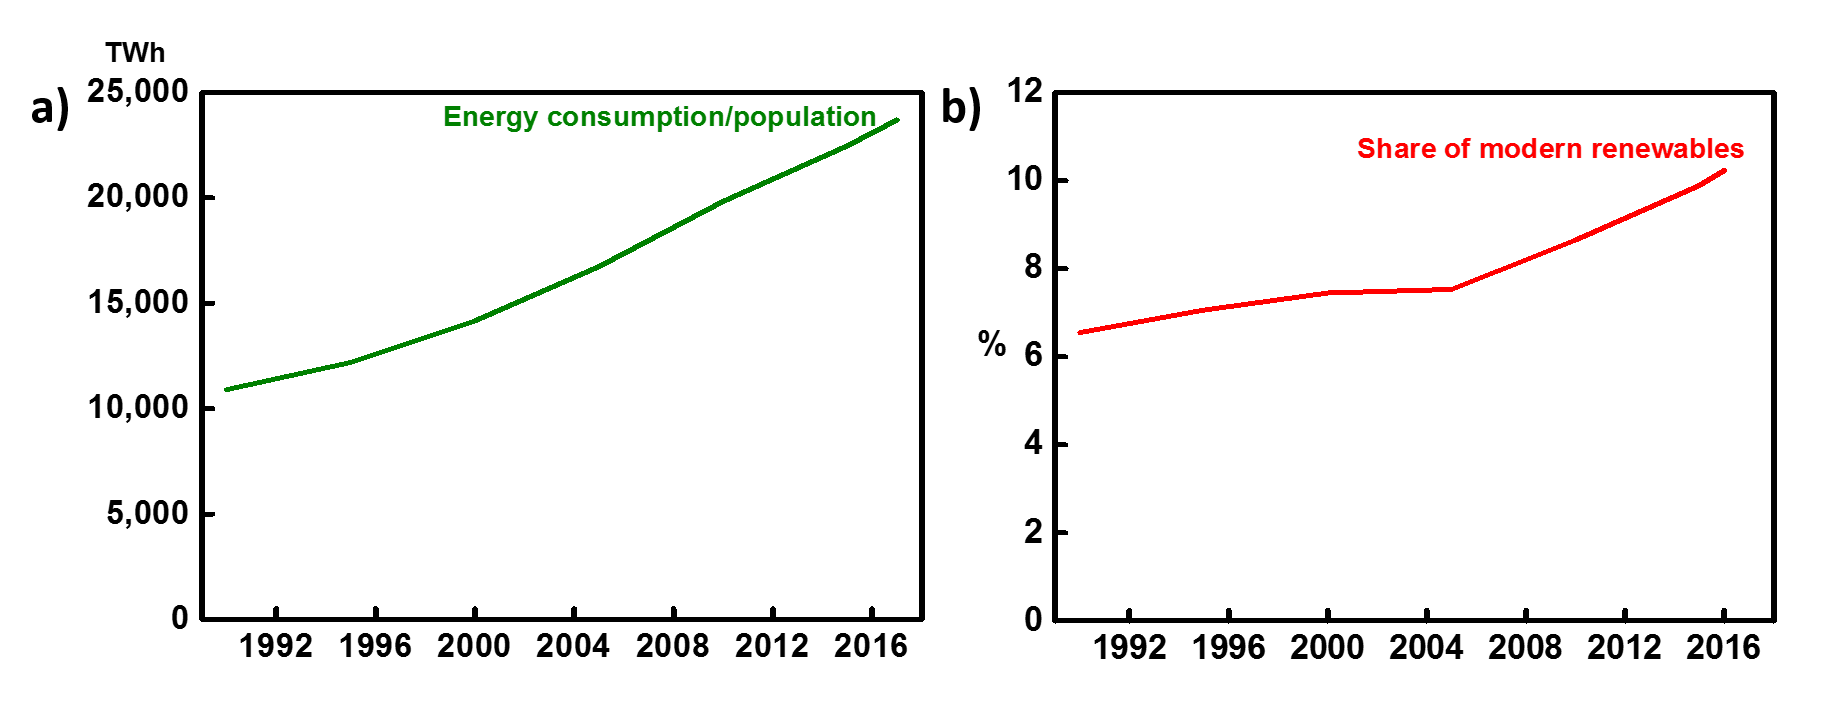
\includegraphics[width=\textwidth]{Figures/chap1fig/IEC2}
\caption{Based on International Energy Agency (IEA) data from 2018 monthly oil data service, www.iea.org/statistics. All rights reserved.}
\label{Figures/chap1fig:IEC2}
\end{figure}

\begin{itemize}
\item \textbf{Battery capacity}: Capacity is the amount of charge or energy stored in a battery. Mathematically, it is evaluated by integrating current over time. The fundamental units of battery capacity is coulombs (C), though Amp-hrs (Ah) is more commonly used.  Theoretical capacity (ideal capacity a battery can store under equilibrium conditions) is calculated with the help of chemical reactions that take place inside the cell. Using Faraday's constant (F = 96,484.56 C mol$^{-1}$), theoretical capacity of a battery can be determined from equation \ref{eq1}:

\begin{equation} \label{eq1}
  \text{Capacity(Ah) = } \frac{n \times F \times 1 \text{ hour}}{3600 \text{ sec}}\\
\end{equation}

where n = number of electrons participating in the chemical reaction \\
F = Faraday's constant\\
\item \textbf{Battery potential}: Voltage is the  most important characteristic of a battery. It is the point (usually in the middle of a discharge curve), where voltage stays for the longest period forming a plateau. Various factors such as electrolyte stability, polarization of the battery (displacement of electrode potential from the equilibrium value) and concentrations of the active species help in determining a cell's voltage. Figure \ref{Figures/chap1fig:CDCforcellvoltage} represents an ideal charge and discharge curve (CDC). To avoid any permanent damage, a battery should not be discharged below a certain level. This voltage is called the "cut-off voltage". Going beyond cut-off voltages (both upper and lower cut-offs) might lead to certain reactions that decompose the electrolyte (also known as side reactions) resulting in an irreversible capacity loss. 

\begin{figure}[tbh!]
\centering
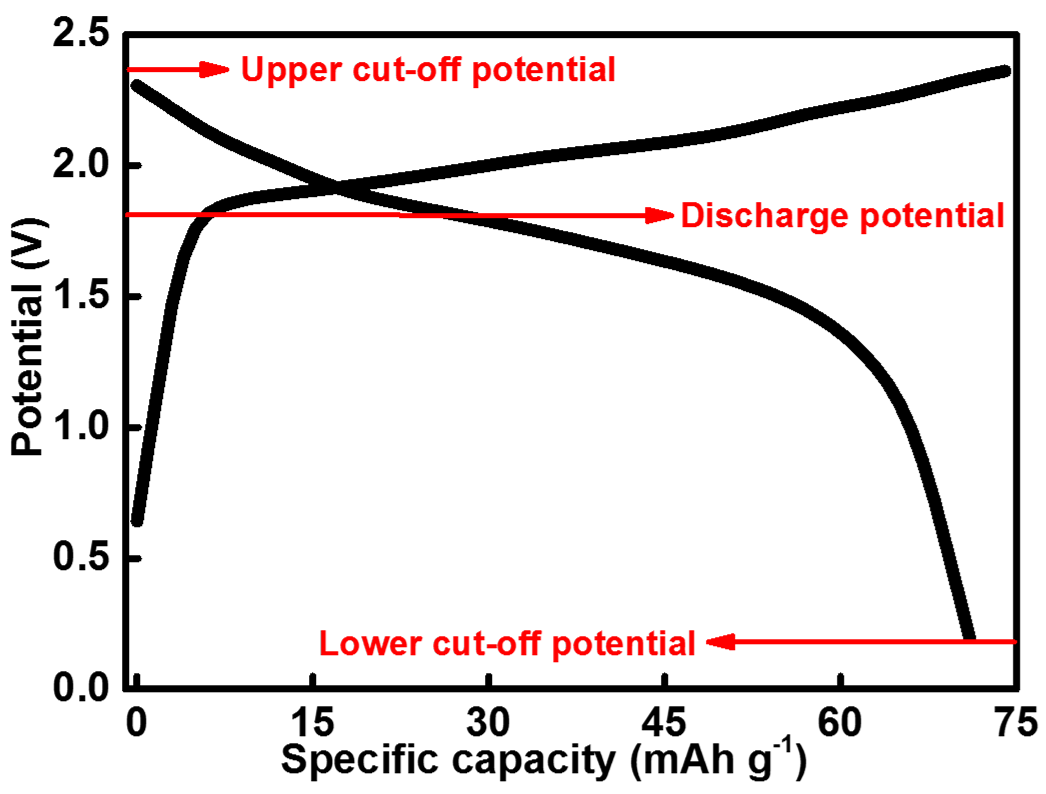
\includegraphics[width=0.75\textwidth]{Figures/chap1fig/CDCforcellvoltage}
\caption{A charge and discharge curve of an aluminium-ion cell using graphite as the cathode and pure aluminium as the anode. The cell was charged and discharged to 2.45 V and 0.2 V respectively.}
\label{Figures/chap1fig:CDCforcellvoltage}
\end{figure}

\item \textbf{Energy density}: The amount of energy stored in a battery per unit mass or volume is called its energy density. Sometimes, heavy batteries are required to move something as large as a car over long distances, therefore they use batteries with high energy density. A simple way to determine the specific energy or energy density of a battery is using equation\ref{eq2}:

\begin{equation} \label{eq2}
    \text{Energy density = } \text{Battery capacity (Ah)} \times \text{Battery voltage (V)}\\
\end{equation}

\item \textbf{Power density}: Power density measures how quickly a battery can deliver energy. Also known as specific power, it is equivalent to the maximum current one can draw from a battery. Units used to describe power density are W kg$^{-1}$ or W m$^{-3}$. The best way to differentiate between energy and power density of a battery is to use an example of a moving car. Energy density determines how 'far' the car will go, whereas power density determines how 'fast' the car will go.

\item \textbf{Coulombic efficiency}: Coulombic efficiency of a battery is the ratio of number of charges that enter during charge to the number that can be extracted from the battery during discharge. A high coulombic efficiency in excess of 95\% is considered a standard value for commercial battery systems. 
\end{itemize}

\textbf{Primary and secondary batteries}: Primary or non-rechargeable batteries produce current immediately when assembled. They have very high energy densities since it is a single-use system. Common types of disposable batteries include zinc-carbon and alkaline batteries. 
\textit{Secondary}, or rechargeable batteries, need to be charged before their first use. Since they are assembled in the discharged state, applying an electric current (during charge) reverses the cell's active materials chemical state. They find extensive use in portable devices as they store energy that can be drawn after every charge/discharge cycle. The most commonly used examples of rechargeable batteries are nickel-cadmium (Ni-Cad), nickel metal hydride (NiMH) batteries and lithium-ion batteries (LIBs).\\

charging and discharging rates affect the battery capacity. If a high discharge current is applied (i.e. the battery is being discharged very quickly) the amount of energy that can be extracted from the battery is reduced and its capacity decreases. This is because only a fraction of the total reactants are converted to other forms, and therefore the energy available for consumption is reduced. Alternately, if a battery is discharged using low current, more energy can be extracted from the battery and its capacity is higher. Temperature of a battery also affects the energy that can be extracted. At a higher temperature, the capacity is typically higher than at a lower temperature. However, intentionally elevating battery temperature is not an effective method as this might decrease battery lifetime\cite{leng_effect_2015, ma_temperature_2018}. 
An ideal battery should be low-cost, charge and discharge indefinitely under high or low current rate, have a long lifetime with high coulombic efficiency (>95\%), and low-self discharge. However, it is difficult to fulfil the above set of requirements. Researchers are building new batteries that might achieve these objectives \cite{slater_sodium-ion_2013,jian_carbon_2015,aurbach_prototype_2000,lin_ultrafast_2015-2}. \\

Table\ref{table1} compares a few characteristics of rechargeable batteries that currently exist in market. 

\begin{sidewaystable}
\centering
\caption{Characteristics of commonly used rechargeable batteries.} \label{table1}
\begin{tabular}{ |p{3.5cm}|p{2cm}|p{2cm}|p{2cm}|p{4.5cm}|p{4.5cm}|}
 \hline 
\textbf{Battery type} & \textbf{In market since} & \textbf{Energy density} & \textbf{Nominal voltage (V)} & \textbf{Applications} & \textbf{Limitations}\\ 
\textbf{} & \textbf{} & \textbf{(Wh kg$^{-1}$)} & \textbf{} & \textbf{} & \textbf{}\\ 
\hline
Lead-acid & 1881 & 30-50 & 2.0 & backup power supplies for telephone and computer centres, grid energy storage, uninterrupted power supply (UPS), marine applications- submarines & Environmental hazard, low energy density, risk of thermal runaway, transportation restrictions\\
Nickel-cadmium (Ni-Cad) & 1960 & 40-80 & 1.2 & portable electronics, toys, cordless telephones & Environmental hazard, low energy density, high self-discharge\\
Nickel-metal hydride (Ni-MH) & 1990 & 60-120 & 1.2 & Consumer electronics, electric vehicles, hybrid cars & Expensive, high self-discharge, high maintenance\\
Lithium-ion (\ce{LiCoO2}) & 1991 & 150-190 & 3.6 & Smartphones, laptops, tablets, digital cameras, hybrid vehicles, electric motorcycles, scooters, bicycles, personal transporters & Safety hazard, risk of thermal runaway, transport restrictions, environmental hazard\\
Lithium-ion (\ce{LiMn2O4}) & 1996 & 100-135 & 3.8 & Same as above & Same as above\\
Lithium-ion (\ce{LiPO4}) & 1999 & 90-120 & 3.3 & Same as above & Same as above\\
Lithium-ion (LiNi$_{x}$Co{$_{1-x-y}$}O$_{2}$, LiNMC) & 2008 & 190-210 & 3.6 & Same as above & Same as above\\
\hline
\end{tabular}
\end{sidewaystable}

\newpage

\section{Lithium-ion battery (LIB)}
Standard potential of a redox reaction determines whether a voltage is generated between a redox reaction or not. If the difference between the standard potentials is positive, then the reaction will proceed spontaneously, or else a voltage is applied so that the reaction can proceed, which is precisely what is needed in a battery. Therefore, standard potential is an important parameter while fining a suitable battery anode\cite{liu_understanding_2016}. Lithium has the most negative electrochemical potential (-3.04 V), which enables it to achieve very high energy and power densities (refer to equation \ref{eq2}). This is the reason why LIBs are a popular battery-choice for most applications.\\
%LIB is a power pack of choice not only on the Earth, but also in space. In October 2019, a few astronauts on board the International Space Station (ISS) stepped outside their quarters for a spacewalk. Flight engineers Christina Koch and Jessica Meir were assigned the task of manually swapping out two nickel hydrogen (NiH) batteries for one brand new LIB. It was the first ever all-female spacewalk in human history! The battery replacement would not only upgrade the station's electrical system but also extend it's life, at least through 2020's. ISS was launched into orbit in 1998 with 48 NiH batteries. The National Aeronautics and Space Administration (NASA) has started swapping these old batteries, since 2017, with 24 new LIBs  that provide higher energy density and a better power efficiency. Naturally, they had to be careful while handling these heavy batteries (195 kg). LIBs come with a potential risk of thermal runaway, which means an increase in temperature leads to conditions that cause a further increase in temperature, often leading to a destructive result. Inside a pressurised oxygen-rich capsule, the results would have been catastrophic! 
The most commonly used electrolyte for LIBs is based on lithium hexafluorophosphate (\ce{LiPF6}) and mixture of carbonate solvents such as dimethyl carbonate (DMC), ethyl methyl carbonate (EMC), or diethyl carbonate (DEC) as they make less viscous electrolyte and enhance its conductivity. However, they are flammable and show flash points around room temperature (between 16 and 33$^{\circ}$C). In combination with an oxidant and an ignition source, they may catch fire and cause explosions! In addition, future battery demand will place increasing pressure on lithium and cobalt reserves\cite{turcheniuk_ten_2018}. To find a suitable alternative, one needs to examine theoretical specific capacities of different ions that can replace lithium. Metals in the upper left corner of the periodic table, such as sodium (Na), magnesium (Mg), potassium (K) and calcium (Ca) report higher theoretical capacities than the others and can be alternatively used as battery anodes. Table  \ref{table2} compares the metrics of a few potential metal anodes. 

\begin{table}[tbh!]
\caption{Comparing important parameters of various metal anodes.} \label{table2}
\begin{tabular}{|ccccccc|}
\hline
 & \textbf{Li} & \textbf{Na} & \textbf{Mg} & \textbf{Al} & \textbf{K} & \textbf{Ca}\\
\hline
\hline
Valence electrons & 1 & 1 & 2 & 3 & 1 & 2\\
Specific capacity (mAh g$^{-1}$) & 3862 & 1166 & 2205 & 2980 & 685 & 1340\\
Standard potential (V) & -3.04 & -2.71 & -2.36  & -1.68 & -2.93 & -2.87\\
Abundance (ppm) & 18 & 22700 & 23000 & 82000 & 18400 & 41000\\
\hline  % Please only put a hline at the end of the table
\end{tabular}
\end{table}

High abundance and easy accessibility of aluminium resources enable aluminium-ion batteries (AIBs), together with their electrochemical characteristics, offer the opportunity to become an ideal alternative.

\section{Aluminium-ion battery (AIB)}
The second most promising metal with a relatively high standard oxidation potential is aluminium (Al). AIBs use aluminium metal as anode, which makes it cost-effective, recyclable, and environment-friendly. A multivalent ion insertion (intercalation) is feasible, which increases the theoretical energy density of AIBs (Table \ref{table2}). Moreover, the high abundance and easy accessibility of Al resources enable Al-ion batteries to become an ideal candidate for large-scale energy storage system. 
The idea to use aluminum in batteries was born in 1800's. Inventors like Joseph Richards and James Sully worked on galvanic batteries using a carbon-aluminum electrode\cite{richards_aluminum_1887, sully_james_1897}. These cells maintained a nearly constant electromotive force (EMF) on closed circuit for several weeks at a time. The negative electrode was externally exposed to air and a mixture of potassium carbonate (\ce{K2CO3}) and kerosene oil was used as the electrolyte. Their motive was to provide an aluminum dry cell with a longer shelf life. Another attempt was made to make commercially viable aluminium batteries in the 1950's. Donald Sargent reported an Al/NaOH and ZnO/\ce{MnO2} system \cite{sargent_voltaic_1951}. Both these systems suffered through similar problems of aluminium passivation leading to very low energy densities and hence could not be commercialised. One of the first aluminum air batteries were reported by Zaromb\cite{zaromb_use_1962} in the 1960s. He found that addition of zinc oxide or ammonium salts to the electrolyte reduced the rate of aluminum corrosion in the strongly basic electrolytes. However, the nature of the stabilization was irregular and sometimes the corrosion rate would experience a sudden increase\cite{bockstie_control_1963}. In 2002, Li \textit{et al.} discovered the reversible electrodeposition of aluminum from both aqueous non-aqueous electrolytes\cite{li_aluminum_2002}. This proved aluminum had the potential to be used as an anode in rechargeable batteries. However, the passivating oxide layer on the anode surface was damaging the battery performance. Its presence caused loss of electrode potential resulting in lower cell potential than the theoretical value. The oxide layer further inhibits cell performance by causing a 'delayed action', which is a time delay during which the cell reaches its operating potential during discharge. This delay is due to the gradual breakdown and removal of the oxide layer from the aluminum anode surface. It not only delayed obtaining reversible potential but also hindered the anode activation. Finally in 2010, Paranthaman \textit{et al.} made the first rechargeable aluminum-ion battery using a cathode composed of \ce{Mn2O4} and an ionic liquid as the electrolyte, based on the works by Jiang \textit{et al.} and Peng \textit{et al.} \cite{paranthaman_transformational_2010-1, jiang_electrodeposition_2006-1,peng_investigation_2008}. The electrolyte was made of aluminium trichloride (\ce{AlCl3}) and 1-Ethyl-3-methylimidazolium chloride (EMImCl) (discovered by Gillford \textit{et al.}) in a ratio of 2:1 \cite{gifford_aluminum/chlorine_1988-1}. The higher concentration of \ce{AlCl3} makes the ionic liquid a Lewis acid, which prevented Al passivation. 
Reversible deposition and dissolution of Al occurs in non-aqueous electrolytes such as molten salts NaCl-\ce{AlCl3} or ionic liquids (quaternary ammonium species) at room temperature with no passive oxide layer formed on the aluminum anode (\cite{vestergaard}\cite{galinski}\cite{elia_insights}). The electrochemical stability window of the ionic liquids enable deposition of Al and increase the cell voltages \cite{li_aluminum_2002}. Ionic liquids consist of weakly coordinated complex ions, which are liquid below 100 C, or at room temperature. Another advantage of the ionic liquids is their wide electrochemical window, ranging from 4.5 to 6.0 V. This makes them suitable for high-performance energy storage devices \cite{wang_binder-free_2015}. In addition, most ionic liquids show a high thermal stability, non-flammability, non-volatility and a low vapor pressure, in comparison to organic solvents. Ionic liquids such as 1-ethyl-3-methylimidazolium (EMIm), 1,3-di-nbutylimidazolium or 1-butylpyridinium, in combination with chloroaluminate (Al$_x$Cl$_y$) anions can achieve a potential window of up to 6 V. Furthermore, they reach an electric conductivity of 10 mS cm$^{−1}$, which is similar to the magnitude of most aqueous electrolytes \cite{ngo_thermal}. Ionic liquids based on \ce{AlCl3}  are mostly hygroscopic \cite{ueda_electro}. A tiny amount of moisture might decompose them or decrease the potential window. The acidity of chloroaluminate-based ionic liquids depends on the molar composition of the anion and cation components, which also affects their conductivity and viscosity \cite{buzzeo}. 
Al deposition (during charge) and dissolution (during discharge) at the anode takes place in a Lewis acidic ionic liquid, containing \ce{Al2Cl7^{-}} (equation \ref{eq3} \cite{galinski}.

\begin{align} \label{eq3}
   4\ce{Al2Cl7^{-}} + 3\ce{e-} \rightleftharpoons \ce{Al} + 7\ce{AlCl4^{-}}  
\end{align}

\ce{Al2Cl7^{−}} anions are formed when the molar ratio of \ce{AlCl3} is higher than 0.5, the ionic liquid becomes a Lewis acid. An excess of the cation results in a Lewis basic ionic liquid, due to the presence of free halide ions (Equation \ref{eq4}) \cite{holbrey}. A Lewis neutral composition consist of the same molar ratio of \ce{AlCl3} and EMImCl. 

\begin{align}\label{eq4}
   2\ce{AlCl4^{-}} \rightleftharpoons \ce{Al2Cl7-}+\ce{Cl-} 
\end{align}

This was a major breakthrough since most of the earlier inventions displayed lower capacity and were not good enough for long term practical use. EMImCl/ \ce{AlCl3} has since been the most commonly used electrolyte for non-aqueous aluminum-ion batteries.
% This was the reason why aluminium batteries were never good enough for long-term practical use. Holleck and Giner studied the electrochemistry of aluminum metal in the \ce{AlCl3}-KCl-NaCl eutectic melt as a possible electrolyte for aluminum batteries with high energy densities. They also found that the aluminum anode was passivated in these melts by formation of a solid salt layer due to local concentration changes at the metal surface during current flow. In addition, the cathodic deposition of aluminum resulted in formation of dendrites and production of chlorine gas\cite{holleck}. The oxide layer of an aluminum anode caused a number of problems preventing these cells from commercialisation. 
Figure \ref{Figures/chap1fig:AIBmech} illustrates an AIB using an ionic liquid  (made EMImCl/\ce{AlCl3}) electrolyte and 99\% pure Al foil as anode.

\begin{figure}[tbh!]
\centering
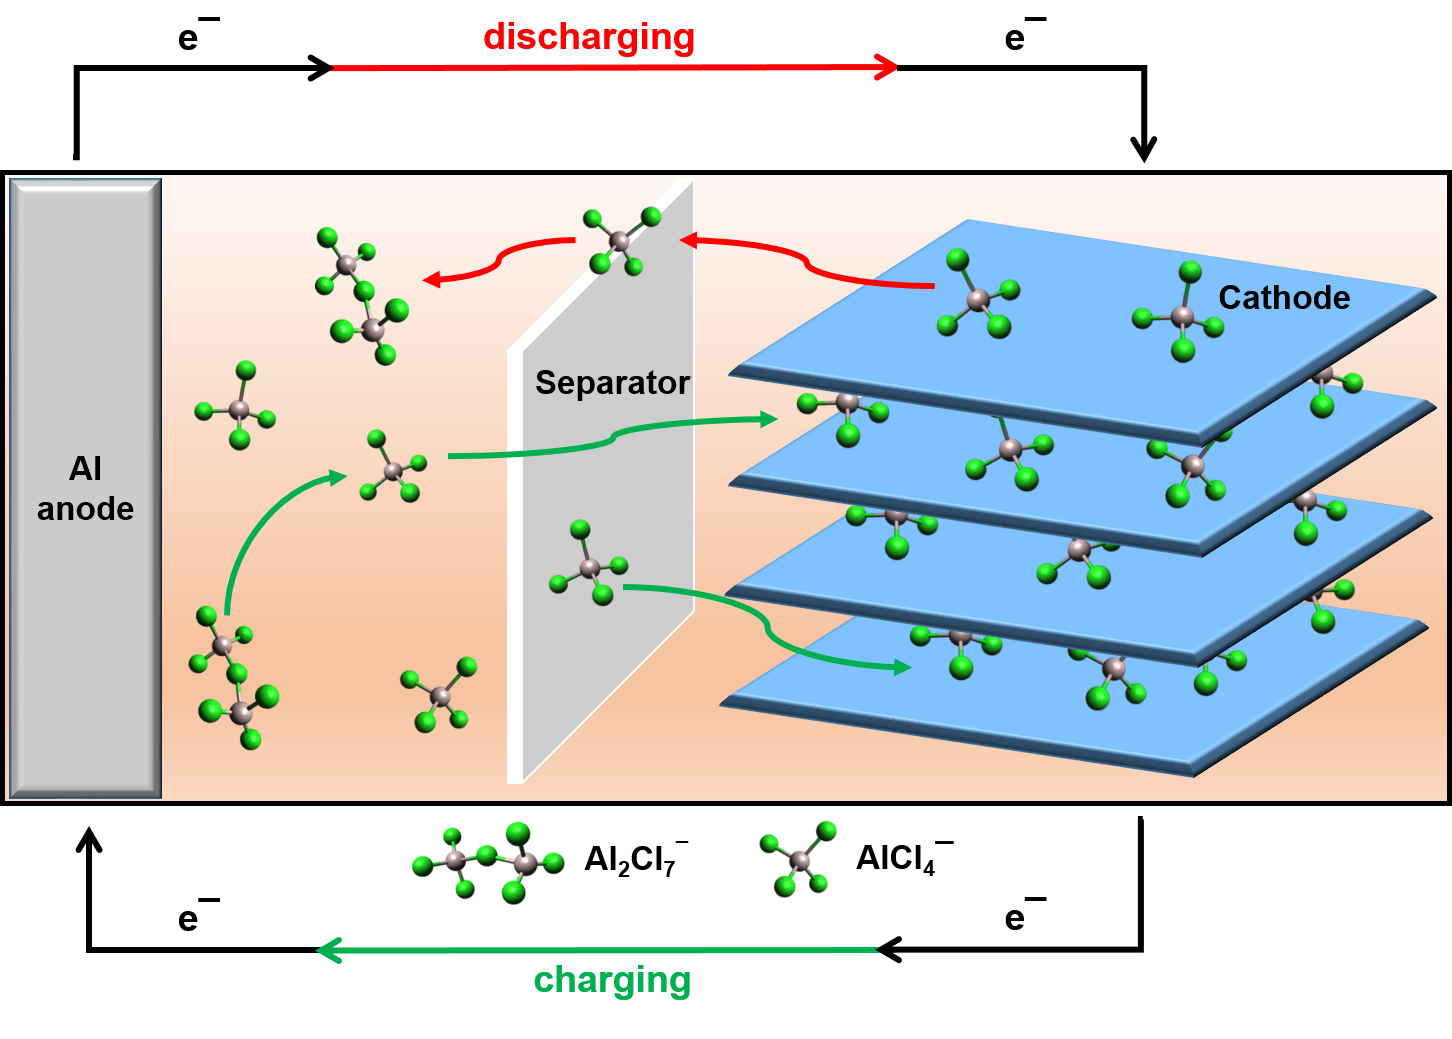
\includegraphics[width=0.75\textwidth]{Figures/chap1fig/AIBmech}
\caption{A schematic representation of a non-aqueous aluminium-ion battery (AIB).}
\label{Figures/chap1fig:AIBmech}
\end{figure}\\

An electrolyte is a chemical medium that allows the flow of charge between the cathode and anode. It promotes movement of ions from the cathode to the anode. It is usually made of soluble salts, acids or other bases in liquid, gelled or dry media, a polymer, or ionic liquids, also known as molten salts \cite{xu_nonaqueous_2004,armand_ionic-liquid_2009,croce_nanocomposite_1998}. The ions transport current through the electrolyte, while the electrons flow in the external circuit generating an electric current.

\subsection{Aqueous aluminium-ion batteries (AAIBs)}
Using water as an electrolyte would reduce the battery costs significantly and increase battery safety. However, these batteries come with their own set of problems. 

\begin{itemize}
    \item the electrochemical plating/stripping of aluminium occurs at a voltage far from the stable potential window of water
    \item aluminium trichloride \ce{AlCl3} is highly acidic and might result in dissolution of active material leading to corrosion of battery parts
    \item a cathode material with a good cycling stability is yet to be discovered
\end{itemize}  

Anatase titanium oxide (\ce{TiO2}) has been investigated as an intercalation electrode for AAIBs. \ce{TiO2} nanostructures have been commonly used as cathode materials in aqueous AIBs. Improving characteristics such as cycle life, efficiency and rate capability would enable these batteries to be used for high power applications. However, limited focus has been given to cycle life, efficiency and rate capability in the recent aqueous Al-ion literature. Cycling data for \ce{TiO2} nanotubes were presented up to cycle 13 by Liu et al \cite{liu_aluminum_2012}.  %Recently, a graphene enhanced \ce{TiO2} electrode was shown to produce a capacity between 10 and 25 mAh g$^{-1}$ at a current density of 6.25 A g$^{-1}$. However, only 125 cycles were possible and coulombic efficiency was observed to be very low at approximately 50\%. Similarly, the charge discharge profiles observed for the nanospheres and nanotubes show low coulombic efficiencies of around 80-85\%. The reason for low efficiency of \ce{TiO2} in aqueous AIB electrolyte is yet to be explored, but the possibilities could be oxidation of \ce{Ti3+} due to dissolved \ce{O2} in electrolyte, \ce{H2} gas evolution or an irreversible reduction of \ce{Ti4+} to \ce{Ti2+} while charge.  
Aluminium in aqueous systems instantaneously forms a very thin (thickness $\sim$2-10 nm) surface layer of \ce{Al2O3} \cite{vargel_translated_2004}. This layer is stable over a pH range of about 4.0-8.6. Although formation of a surface film on an Al current collector would be an advantage in LIBs, it provides a barrier for dissolution of Al and transportation of \ce{Al^{3+}} ions in AIBs \cite{myung_electrochemical_2011}. This is why AAIBs fail to achieve high energy densities for long-term practical use.

\subsection{Non-aqueous AIBs}
As discussed in Section 1.2, chloroaluminates (Al$_x$Cl$_y$) have been known for aluminium electrodeposition since the 1970s and have been used as electrolytes for rechargeable aluminium batteries\cite{weppner_ionic_1976, fung_reaction_1972}. Systems with a general formula MCl-\ce{AlCl3} where \ce{M+} can be a cation like \ce{Na+}, \ce{Li+} or an organic species like pyrrolidinium or imidazolium have been tested as electrolytes for rechargeable AIBs\cite{das_aluminium-ion_2017}. These melts can be acidic, basic or neutral. In the acidic systems, the dominant species is \ce{Al2Cl7^{-}}, while in a basic system \ce{Cl-} and \ce{AlCl4^{-}} anions coexist whereas in neutral melts, only \ce{AlCl4^{-}} anions exist. Since the standard electrode potential of \ce{Al^{3+}}/Al (-1.68 V) is lower than \ce{H+}/\ce{H2}, evolution of \ce{H2} gas occurs when Al foil reacts with aqueous acid or alkali solution. Thus, Al cannot be electrochemically striped or deposited in a common aqueous solution. To be compatible with Al anode, the ionic liquid \ce{AlCl3}/EMImCl, which has a wider electrochemical active window, emerges as the typical electrolyte. It provides a mild corrosive effect on the anode surface to activate the Al striping and plating reaction. 

\begin{align*}
        \ce{Al} + 7x\ce{AlCl4-} \rightleftharpoons 4x\ce{Al2Cl7-} + 3x\ce{e-}
\end{align*}

Not only they overcome the above mentioned problems with AAIBs, \ce{AlCl3}/ imidazolium ionic liquids are the quintessential electrolytes for non-aqueous AIBs making them much safer than LIBs \cite{jayaprakash_rechargeable_2011, lin_ultrafast_2015-3,wang_new_2013-1,rani_fluorinated_2013}. 

\section{Cathodes for secondary batteries}
A usable cathode material should have certain properties: good conductivity, high natural abundance, stability in the presence of an electrolyte, good working voltage, and a large reversible storage capacity obtainable at that potential. In addition, it should be easy to fabricate. Theoretical capacity of a cathode material can be found using equation:

\begin{equation} \label{eq5}
   C_{t} \text{ = } \frac{n \times F}{3.6 \times M}
\end{equation}\\
where n = number of reactive electrons per formula unit,\\
M = molar weight of the cathode material and\\
F = Faraday constant\\
\ref{eq5} implies that a material with a low molecular weight and high number of reactive electrons would deliver a high theoretical capacity.

\begin{figure}[h!]
\centering
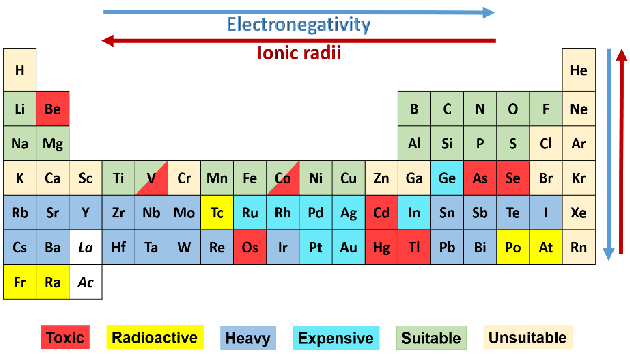
\includegraphics[width=\textwidth]{Figures/chap1fig/pertab}
\caption{The periodic table suggesting elements that can be used as battery materials. However, a few elements from this table have shown good electrochemical performance such as Mo, Sn, Nb and W. Potassium and calcium-ion batteries have also been studied.}
\label{Figures/chap1fig:pertab}
\end{figure}\\

Figure \ref{Figures/chap1fig:pertab} displays the elements that can be used for designing new cathodes. Transition metals have variable valence states; this increases the number of electrons that can be stored, increasing the battery capacity. However, some transition metals such as vanadium (V) and cobalt (Co), despite their toxicity, have been tested and are being used as cathode materials in LIBs.
%The type of bond formed between a metal ion and the ligand plays an important role in determining the electrochemical potential of the material. When the electronegativity difference between the two is high, an ionic bond is formed. A smaller difference results in a covalent bond. Materials with a covalent bonds form poorly packed structures, while ionic bonds form dense structures. A stable structure would enhances the phase stability and electrochemical potential of the material \cite{melot_design_2013}. Furthermore, electrode potential depends on the ionic radius of the material. When an atomic nuclei is loosely bound to its valence electrons, the system needs lower energy for electron transfer , which leads to a lower potential. If more energy is consumed during electron transfer  for materials having a lower ionic radii, the electrochemical potential of the material increases. 
Using Nernst equation
\begin{equation} \label{eq6}
    -\Delta G \text{ = } n \times F \times E
\end{equation}\\
where $\Delta$G = change in internal energy during ion intercalation,\\
n = number of electrons stored per formula unit,\\
F = Faraday constant and\\
E = electrochemical potential of the material, it was realised that the electrochemical potential is affected by interaction between atoms or electrons that change the internal energy. Using polyanionic ligands such as phosphates, sulfates and silicates, which are more electronegative, results in formation of ionic bonds \cite{liu_understanding_2016}. This further enhances the electrochemical potential of a material \cite{melot_design_2013}. For example, \ce{LiCoPO4} (polyanionic) displays a higher potential at 4.8 V than \ce{LiCoO2} (oxide), which has a potential at 4.0 V\cite{masquelier_polyanionic_2013}. 

\subsection{Cathodes for non-aqueous AIBs}
Based on the structure and reaction mechanisms, cathodes can be categorised in two ways.\\
\textbf{Carbon-based materials} have a high surface area. Graphite, a form of carbon with hexagonal structure, has been commonly used as an electrode in various battery systems. It has a layered structure (that enhances the intercalation process), good thermal and electrical conductivity, and a high electrical potential \textit{vs.} \ce{Al}/\ce{Al^{3+}} of 2.1 V. Different forms of graphite have been used in AIBs. An AIB using graphene nanoribbons on highly porous three-dimensional (3D) graphene foam as cathode reported the highest capacity of 148 mAh g$^{-1}$. Fluorinated graphite \cite{rani_fluorinated_2013}, kish graphite flakes \cite{wang_kish_2017-1}, 3D graphitic-foam \cite{wu_3d_2016}, graphene aerogels\cite{huang_graphene_2019} and several other forms have been tested, which showed discharge capacities ranging from 60-250 mAh g$^{-1}$. In graphite-based batteries, Al$_x$Cl$_y$ anions intercalate into the graphitic layers when the cell is being charged and deintercalate during discharge. Electroplating and dissolution of Al takes place at the anode.\\
Activated carbon, owing to its highly porous structure, provides a high surface area and renders an additional capacitor-like charge storage, where absorption of electrolyte ions takes place on the cathode's surface \cite{eliad_ion_2001, zhu_carbon-based_2011-2}.\\
The second type of cathode materials are \textbf{two-dimensional (2D) materials} such as transition metal dichalcogenides (TMDs), transition metal oxides (TMOs), MXenes, Prussian blue analogues (PMAs), and a few other metallic oxides. These materials offer tunable chemical and physical properties due to their various elemental compositions and different crystallographic structures. In addition, they possess excellent electrochemical properties \cite{chia_electrochemistry_2015}. A 2D plane imparts a high surface area, which allows complete utilization of all available sites in a cathode material \cite{jia_interfacial_2016,naguib_mxene_2012}. Each metal in a TMD is coordinated with two chalcogens; the metal in in +4 oxidation state while the chalcogen atom is in -2 state. Interaction or insertion of ions from the electrolyte alters the oxidation states of the molecules resulting in redox process. In addition, a few TMDs, especially molybdenum (Mo) and tungsten (W) dichalcogenides, are capable of phase transition after ion insertion. Due to introduction of extra electrons and rearrangement of d orbitals, a phase transition from 2H to 1T takes place \cite{acerce}. This changes the electronic properties of the material since 2H \ce{MoS2} is semiconducting, while 1T \ce{MoS2} is metallic. For the above mentioned reasons, 2D materials have gained enormous attention in recent years. 
%These materials have promoted a relatively reversible trivalent reaction. Strong electrostatic nature of trivalent \ce{Al^{3+}} sometimes leads to sluggish kinetics, high over-potentials, and degradation of the host structure. Therefore, to accommodate the highly charged ions, it is essential for the cathode materials to possess weak bond strengths between the host frameworks. Our unpublished, preliminary density functional theory (DFT) calculations indicated a significant decrease in inter-layer spacing of these materials when \ce{Al^{3+}} cations were assumed to intercalate (owing to the very high charge density of \ce{Al^{3+}}). Therefore, we propose intercalation of \ce{AlCl4-} anions into the layered cathode. XRD, Raman spectroscopy and XPS were used to verify our hypothesis.
During this study, various carbon-based and 2D materials were tested as potential cathodes for rechargeable non-aqueous AIBs. The results have been reported in the subsequent chapters.

\section{Research objectives}
The goal of this PhD project is to find new cathodes for rechargeable AIBs that perform better than state-of-the-art. 
\begin{itemize}
    \item Molybdenum dichalcogenides, a few transition metal oxides or sulfides, boron nitride (inorganic graphite) would undergo a similar mechanism and deliver a stable performance. 
    
    \item Materials with high surface area such as activated carbon or nano-structured materials, provide a better contact between the cathode and the electrolyte, thus have proven to be good battery materials. They provide a faster and an efficient pathway for electron diffusion, which improves the kinetics of the system and increases the battery's energy density. We tested high surface-area materials such as activated carbon, carbon black, nanostructures of molybdenum dichalcogenides, as cathodes for non-aqueous AIBs to confirm our hypothesis.
    
    \item Once a cathode achieves high capacity (> 60 mAh g$^{-1}$), and a high voltage (> 1.0 V), it is equally important to establish its mechanism. This would help in designing a better cathode. X-ray diffraction studies, Raman spectroscopy, and X-ray photoelectron spectroscopy are a few techniques that have been used to analyse cathode materials. 

\end{itemize}






